%	% ****** Start of file MolecularSpinFlipLoss.tex ******
%
%
%

\documentclass[%
 reprint,
%superscriptaddress,
%groupedaddress,
%unsortedaddress,
%runinaddress,
%frontmatterverbose,
%preprint,
%showpacs,preprintnumbers,
%nofootinbib,
%nobibnotes,
%bibnotes,
 amsmath,amssymb,
 aps,
prl,
%pra,
%prb,
%rmp,
%prstab,
%prstper,
%floatfix,
]{revtex4-1}


\usepackage{graphicx}% Include figure files
\usepackage{dcolumn}% Align table columns on decimal point
\usepackage{bm}% bold math
\usepackage[hidelinks]{hyperref}% add hypertext capabilities
%\usepackage[mathlines]{lineno}% Enable numbering of text and display math
%\linenumbers\relax % Commence numbering lines
\usepackage{textcomp}
%\usepackage{polish}
\usepackage[utf8]{inputenc}
\usepackage{color}
\newcommand{\red}[1]{{\color{black} #1}}

% Define new commands for common phrases and standardized typesetting
\newcommand{\exmple}{This is an Example.}



\begin{document}

\title{Beyond the Limits of Conventional Stark Deceleration}%

\author{David Reens}
\thanks{dave.reens@colorado.edu}
\altaffiliation{Present Address: Lincoln Laboratory, Massachusetts Institute of Technology, Lexington, Massachusetts 02420, USA}


\author{Hao Wu}
\thanks{hao.wu@colorado.edu}
\altaffiliation{Present Address: Department of Physics and Astronomy, University of California, Los Angeles, California 90095, USA}

\author{Alexander Aeppli}
\author{Anna McAuliffe}

\author{Piotr Wcis\l o}
\altaffiliation{Present Address: Institute of Physics, Faculty of Physics, Astronomy and Informatics, Nicolaus Copernicus University, Grudzi\k{a}dzka 5, PL-87-100 Toru\'n, Poland}

\author{Tim Langen}%­
\altaffiliation{Present Address: 5. Physikalisches Institut and Center for Integrated Quantum Science and Technology (IQST), Universit\"at Stuttgart, Pfaffenwaldring 57, 70569 Stuttgart, Germany}

\author{Jun Ye}
\affiliation{JILA, National Institute of Standards and Technology and the University of Colorado and\\ Department of Physics, University of Colorado, Boulder, Colorado 80309-0440, USA}


\date{\today}

%%%%%%%%%%%%%%%%%%%%%
% OUTLINE 
%%%%%%%%%%%%%%%%%%%%%
% Introduction
% Effective Moving Trap
% Alternate Charging Technique
% Experimental Validation
% Further Simulation Results


%%%%%%%%%%%%%%%%%%%%%
% ABSTRACT
%%%%%%%%%%%%%%%%%%%%%
\begin{abstract}
Stark deceleration has enabled the production of cold and dense molecular beams for applications in numerous trapping and collisional studies. Improving the efficiency of Stark deceleration has been actively pursued in order to realize its full potential. One of the chief limitations arises from the transverse focusing properties of Stark decelerators. We introduce a new operation strategy that circumvents this limit without any hardware modifications, and verify our results for hydroxyl radicals. Improved focusing results in a recovery of gains in molecule yield with increased operating voltage, formerly limited by transverse-longitudinal coupling. At final velocities sufficiently small for trapping, molecule flux improves by a factor of four, and potentially more with increased voltage. The improvement is more significant for less readily polarized species, thereby expanding the class of candidate molecules for Stark deceleration.
\end{abstract}

\maketitle


%%%%%%%%%%%%%%%%%%%%%%%%%%%%%%%%%
%     INTRODUCTION
%%%%%%%%%%%%%%%%%%%%%%%%%%%%%%%%%
%\section{Introduction}
Over the past two decades, Stark deceleration has enabled groundbreaking collisional~\cite{Sawyer2011,Kirste2012,Gao2018} and spectroscopic~\cite{Veldhoven2004,Hudson2006,Lev2006,Fast2018} studies of a variety of species~\cite{VanDeMeerakker2012}. 
Subsequent trap-loading~\cite{Bethlem2002,Sawyer2007} greatly enhances interrogation time for such studies~\cite{Sawyer2008} and opens the door for further manipulation~\cite{Reens2017}. 
Alongside the history of achievements enabled by Stark deceleration runs a parallel ongoing saga surrounding their efficient operation. 
Many important steps have been made, not only in understanding the flaws of the canonical pulsed decelerator~\cite{VanDeMeerakker2006,Sawyer2008a}, but also in addressing them through the use of overtones~\cite{VanDeMeerakker2005a,Scharfenberg2009}, undertones~\cite{Zhang2016}, or even mixed phase angles~\cite{Parazzoli2009,Hou2013}. 
Even with these advances, outstanding inefficiencies of the pulsed decelerator, particularly with regard to transverse phase stability, have motivated alternative geometries such as interspersed quadrupole focusing~\cite{Sawyer2008a} and traveling wave deceleration~\cite{Osterwalder2010,VandenBerg2014,Fabrikant2014}.
Although traveling wave deceleration takes a strong step toward truly efficient operation, it comes with significant engineering challenges. 
These may be partially addressed by the combined use of pulsed and traveling wave devices~\cite{Quintero-Perez2013}, or even using traveling wave geometry with pulsed electronics~\cite{Hou2016,Shyur2017}. 
In Zeeman deceleration, a parallel story has unfolded, with early demonstrations~\cite{Vanhaecke2007,Narevicius2008} later improved through the use of anti-Helmholtz configurations with better transverse focusing properties~\cite{LavertOfir2011,Dulitz2014}.
Lacking a comparable breakthrough for Stark devices, others have continued to pursue brand new geometries~\cite{Wang2016}, or even combine the best features of Stark and Zeeman approaches in a single device~\cite{Cremers2017,Plomp2019}.
Our strategy works with conventional geometry and electronics for Stark decelerators, but fully resolves transverse challenges and offers gains even at low speed.

The strategy is to admix new field distributions into the deceleration process that feature strong restoring forces in the transverse directions.
Depending on which field distributions are chosen, we specify two operating modes employing this strategy: focusing (F) and strong focusing (SF).
In the conventional strategy, only two field distributions are used, and one is identical to the other up to translation and rotation.
These field distributions require an electrode array with the capability to apply three distinct equally spaced voltages, usually labeled plus, ground, and minus.
Both F and SF use distributions that may be generated simply by rearranging how the usual three voltages are applied to the decelerator electrodes.
Although F mode is less efficient than SF, it has the unique advantage of requiring no hardware modifications.
SF mode significantly outperforms F mode in simulation, but requires the ability to apply all three voltages to a single electrode.
This is something the conventional mode avoids, and is challenging to implement with existing high-voltage switches.

\begin{figure*}[t!]
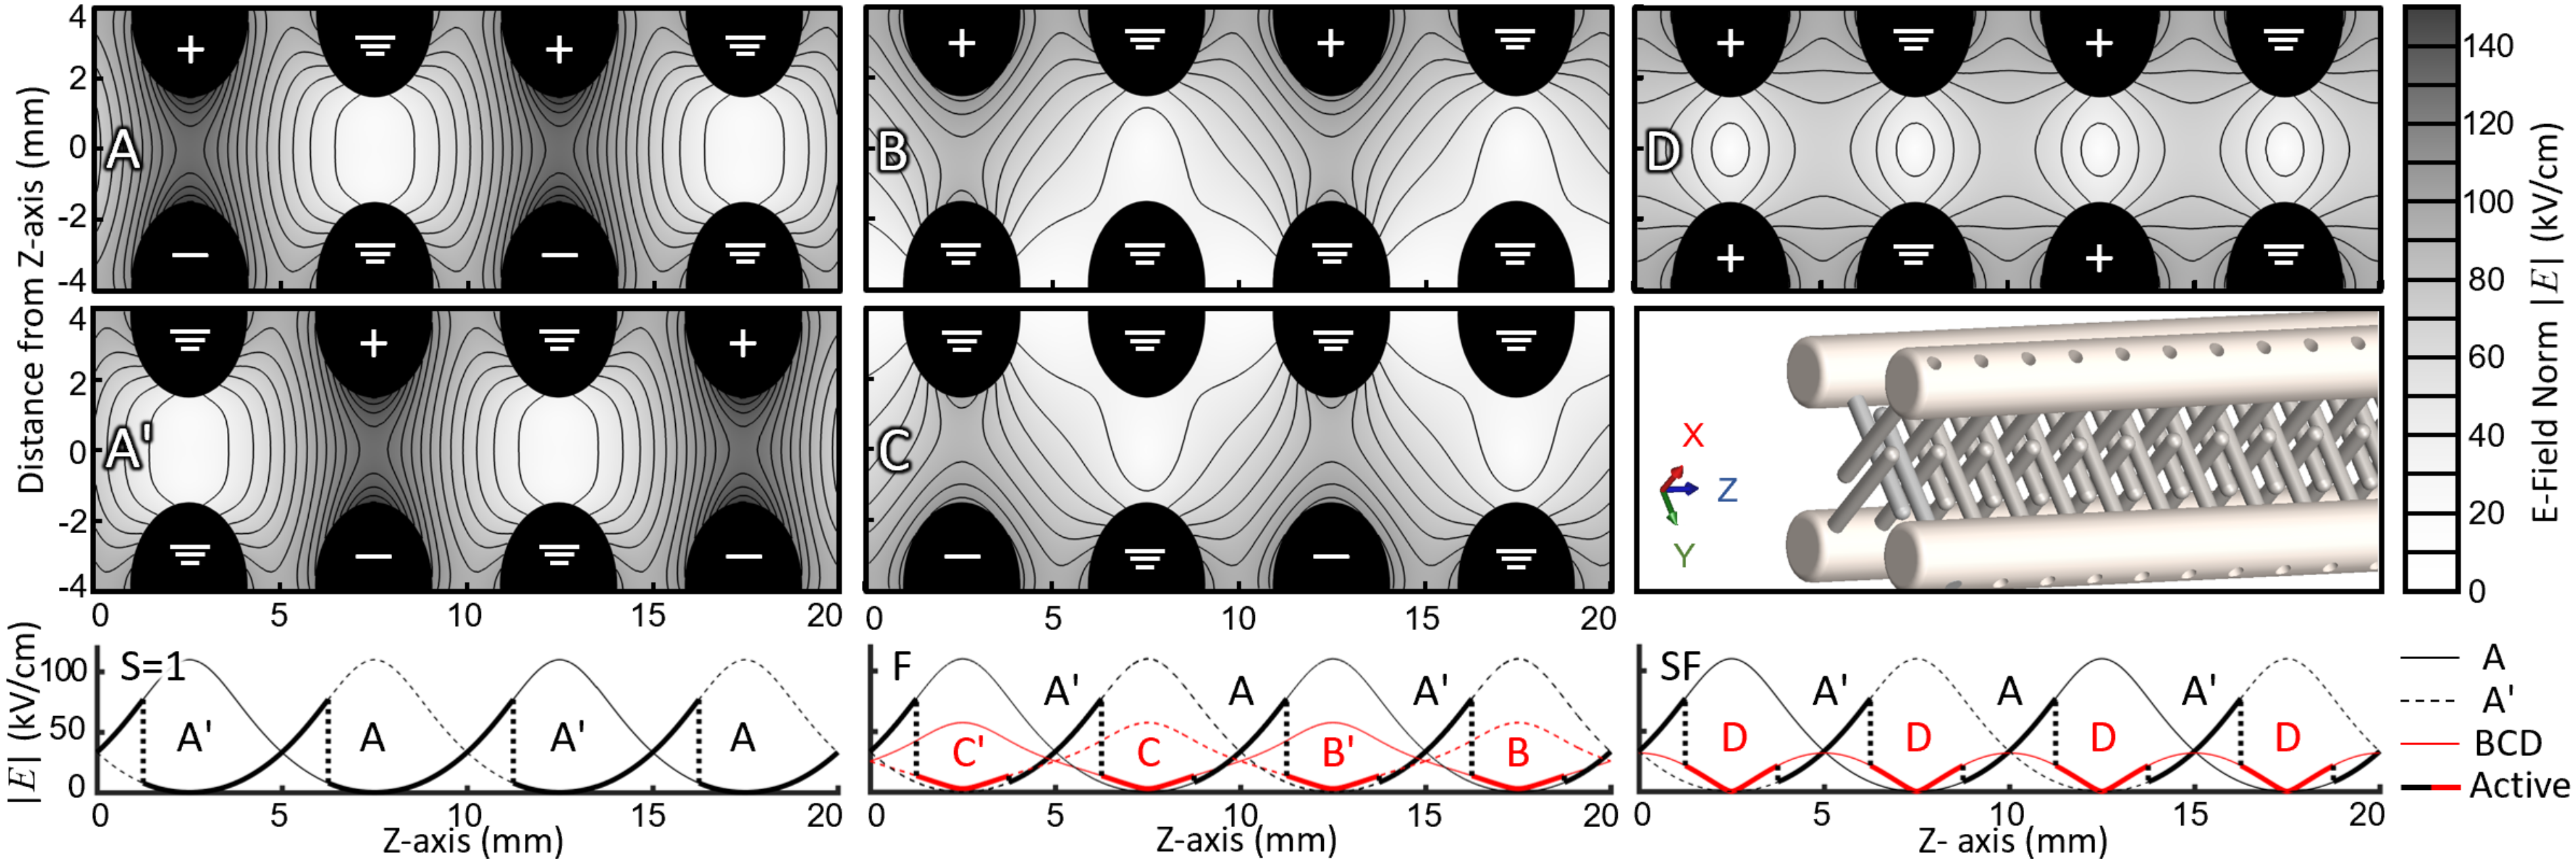
\includegraphics[width=\linewidth]{fig1.png}%
\vspace{-2mm}
\caption{
A new strategy for Stark deceleration, consisting of electric field distributions with transverse focusing (top, middle), 3-d decelerator render(middle-right) and operation modes which employ them (bottom). 
The decelerator consists of four rods, with opposite rods supporting parallel pins.
Distributions are generated in COMSOL with $0$, $+12.5$, or $-12.5$ kV applied to the pins as indicated; the chosen cut plane includes the decelerator axis and is $45^\circ$ to all pins (x-y axis) to ensure their visibility.
The operation modes are specified via on-axis energy diagrams that indicate which distribution is active (bold) as a function of the synchronous molecule's position on that axis.
Left: the conventional distributions A, A$'$ and operating mode S\,=\,1~\cite{VanDeMeerakker2005a}.
Prime indicates a translation of the field configuration along the axis by one pin pair, together with a $90^\circ$ rotation about that axis, since successive pin pairs are always rotated by this amount to ensure confinement in both transverse directions.
Center: distributions B, C and mode F.
Right: distribution D and mode SF.
Distribution D shows clear focusing between grounded pin pairs near $7.5$~mm, evidenced by the electric field norm increasing off axis.
Distributions B, C are less visibly focusing near $7.5$~mm, but taking them together, which is equivalent to traveling through several pin pairs, their average influence is focusing.
Distribution A only focuses near $2.5$~mm, but in fact A$'$ is active in this region.
\vspace{-4mm}
}
\label{fig:chargecartoon}
\end{figure*}
%Modes SF and VSF are not implemented in this work, but could be achieved with a new high voltage system for additional significant enhancement factors according to our simulations, see Fig.~\ref{fig:efftrap}.
%With some investment in high voltage equipment, it may be possible to implement SF mode, providing an additional significant gain even at trappable speeds. %which requires a tri-state switch capable of double the usual switching frequency~\footnote{Behlke HTS-301-151-SiC, options HFB, ILC, ALL-OFF-BIPOLAR.}, so as to make use of the field distribution arising from charging both pins in a pair to the same nenzero voltage.
%A comparable investment would enable VSF mode, but we do not pursue this since it is less useful for trapping, our primary emphasis, for reasons discussed below.
%The slowest speeds shown are suitable for trap loading~\cite{Sawyer2008}.
%Hold times vary from $2-4\text{ ms}$ as final speed is tuned, and thus are in agreement with the simulation results reported for $3\text{ ms}$ in Fig.~\ref{fig:efftrap}.

To understand the mechanism for success of this new strategy, we revisit the operation of a decelerator; Fig.~\ref{fig:chargecartoon} details field distributions and the operating modes derived from them.
In the conventional S\,=\,1 strategy~\cite{VanDeMeerakker2012}, as low-field seeking molecules approach a charged pin pair, they are polarized by the strong electric field and exchange kinetic energy for internal potential energy, effectively climbing a potential hill (Fig.~\ref{fig:chargecartoon}, bottom).
The strong field is then abruptly removed before the molecules have a chance to regain kinetic energy. It is customary to discuss the behavior of an idealized ``synchronous molecule'' that travels along the decelerator axis with zero transverse velocity.
The switching is timed so that the synchronous molecule loses some fixed energy per switch.
It is essential that the synchronous molecule travel only partway up each hill, so that molecules that are ahead of the synchronous molecule get more energy removed, and vice versa.
This creates a longitudinal restoring force for the molecules, centered on the synchronous molecule.
Transversely, restoring force is not inherited from switching events but arises directly from the focusing properties of field distributions.
We speak of these restoring forces in a time-averaged sense, where the high speed of the molecules validates the approximation that the large variation in force that all molecules experience while transiting a single deceleration stage has a negligible effect compared to the average force per stage.
In this approximation, these forces generate a ``traveling trap'' for the molecules~\cite{Bethlem2000}, which translates along the device and decelerates according to a ramp of the switching frequency.

Conventionally, pins are always charged in bipolar pairs, in which case transverse focusing occurs between the charged pin pair, but not significantly elsewhere (Fig.~\ref{fig:chargecartoon}A).
Molecules do not regularly access the focusing region, since pins must always be grounded before the synchronous molecule reaches them to generate a longitudinal restoring force.
As the molecules pass between grounded pins, the transverse field is actually slightly defocusing~\footnote{This is not highly apparent in Fig.~\ref{fig:chargecartoon}A and A', where a $45^\circ$ slicing plane is chosen for visual clarity. The defocusing is strongest in the plane including the decelerator axis that is also normal to the cylindrical axis of the grounded pins.}.  Their transverse confinement also varies with how strongly the molecules are decelerated, and with their distance from the synchronous molecule along the decelerator axis. Such a dependence of transverse confinement on longitudinal position is known as transverse-longitudinal coupling, and it gives rise to the situation that molecules which are coldest longitudinally are less well confined transversely.
The use of deceleration overtones~\cite{VanDeMeerakker2005a} (S\,=\,3, 5, ... ) alleviates	coupling by allowing molecules to fully transit between charged pin pairs regardless of their relative position with the synchronous molecule. This mode of operation leverages the full focusing properties of the conventional field distribution, but at the expense of only using 1/3 of the pin pairs (S=3) for removing energy.

We introduce new field distributions with strong transverse restoring forces when the synchronous molecule is between grounded pin pairs, but retain the use of the conventional distribution otherwise. Field distributions that focus between grounded pins can be created by charging the neighboring pins to voltages that do not sum to zero.
Field lines must then extend toward the grounded pin pair, creating a focusing 2D quadrupole structure.
Possibilities include charging only a single pin (Fig.~\ref{fig:chargecartoon}B, C (F)), or charging both to the same voltage (Fig.~\ref{fig:chargecartoon}D (SF)).

\begin{figure*}[t]
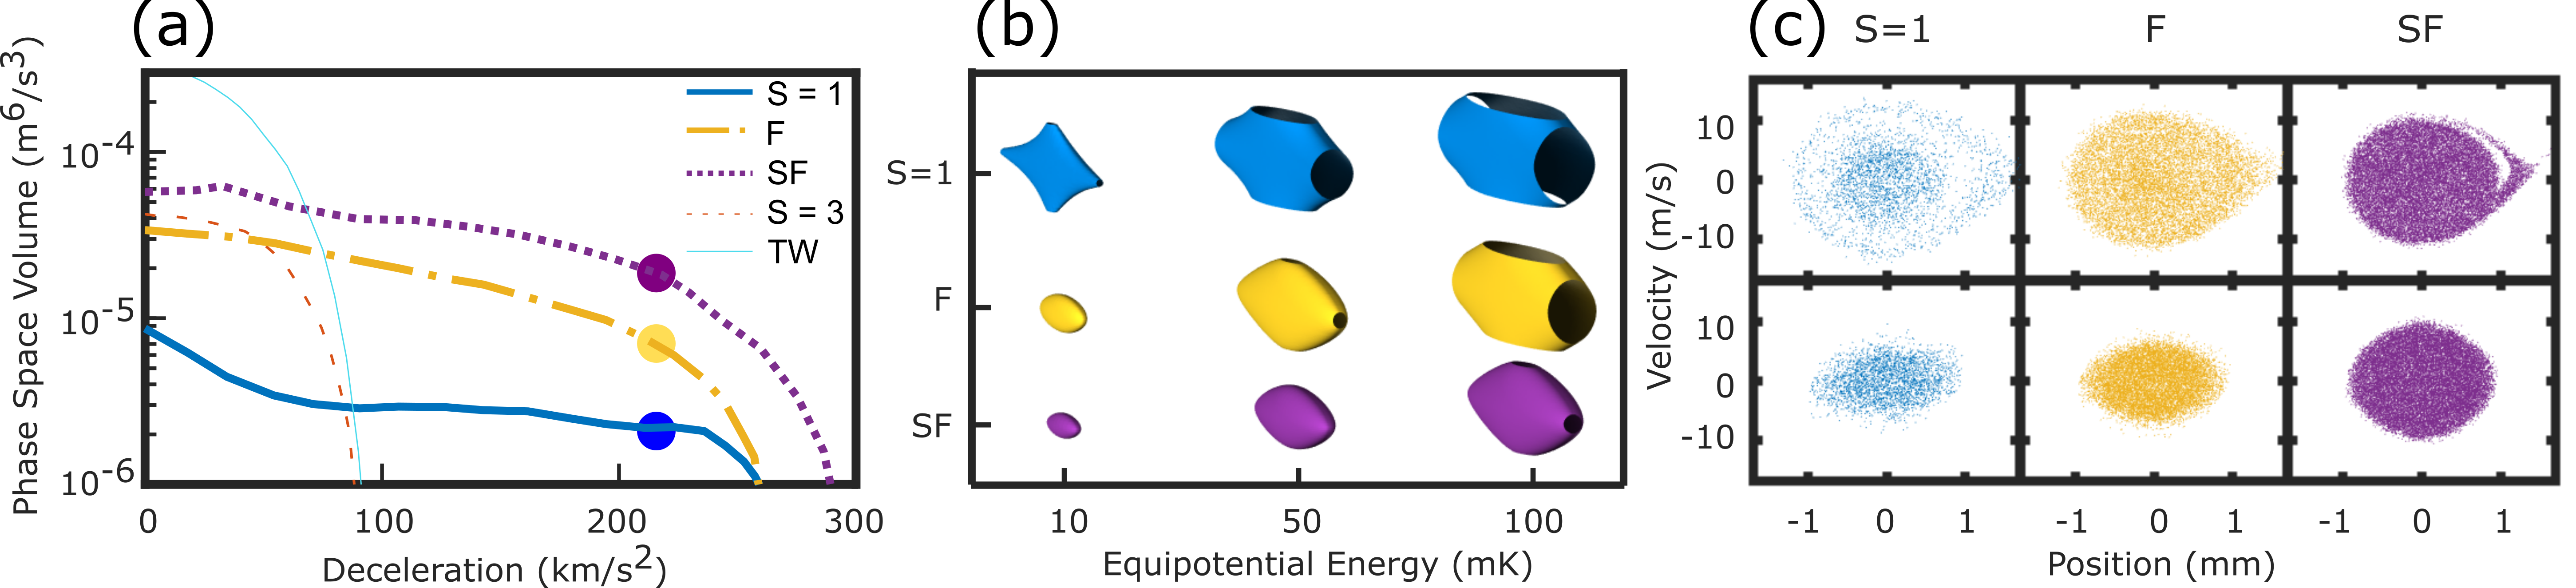
\includegraphics[width=\linewidth]{Figure2.png}%
\vspace{-2mm}
\caption{
Simulation results of different deceleration modes. 
(a) Simulated phase space volume captured by different modes of operation, for varying decelerations and elapsed time fixed at $3$~ms. 
A $10$~kV peak to peak traveling wave (TW) deceleration and $\pm 12.5$~kV S\,=\,3 are also plotted for comparison. 
Three solid dots correspond to the deceleration rate used in panel (b) and (c), respectively. 
(b) Equipotentials of the traveling trap generated for three modes with deceleration fixed at $200 \text{ km/s}^2$. 
Lack of closure of an equipotential indicates the possibility of molecule escape. 
(c) Phase Space Fillings, both longitudinal (top) and transverse (bottom), for the labeled operation modes.
Molecules travel for $3~\text{ms}$ with a deceleration of $200 \text{ km/s}^2$. 
The surviving number of molecules is $3$, $11$ and $24$ thousand respectively. 
Note dramatic improvements in homogeneity and flux, without significant broadening to larger velocity classes.
\vspace{-4mm}}
\label{fig:efftrap}
\end{figure*}
%\section{The Effective Moving Trap}

%In order to quantitatively analyze these operation modes, we directly calculate the traveling trap each sequence generates for the molecules.
In order to best compare these modes in a device-independent way, we perform simulations with fixed travel time ($3$~ms) and varying deceleration rate, see Fig.~\ref{fig:efftrap}(a).
%Simulations are performed as in~\cite{Bethlem2000,Hudson2004} but extended to three dimensions~\cite{ssm}.
%We can inspect the efficiency improvements by calculating the total phase space remaining within the effective traveling well for a given deceleration and time, $3$~ms as in the case of Fig.~\ref{fig:efftrap}a.
S\,=\,1 delivers the smallest phase space volumes, although provides at least some flux even at high deceleration.
Remarkably, F mode offers comparable phase space volume to S\,=\,3, but with triple the deceleration.
SF mode makes more dramatic improvements, extending significant gains to even higher decelerations than possible with any other studied modes.
For the traveling wave (TW) decelerator comparison in Fig.~\ref{fig:efftrap}(a), $10$~kV sine waves are assumed, to our knowledge the largest used to decelerate molecules to rest~\cite{Quintero-Perez2013}. TW offers a good phase-space volume but is limited to a smaller maximum deceleration, similar to S\,=\,3.  
All modes besides TW use the rather small $2$x$2\text{ mm}^2$ open area of our device, while TW devices use rings of $4$~mm inner diameter.
If the new modes were used with a $3\times3\text{ mm}^2$~\cite{Scharfenberg2009} or a $4\times4\text{ mm}^2$~\cite{VandeMeerakker2005} device, phase space volume would increase approximately with the cube of pin pair spacing, and deceleration would decrease linearly since the pin-pair to pin-pair spacing also must increase.
Unlike TW however, the performance of F, SF, and S\,=\,1 all degrade significantly when longitudinal velocity $v_z < 50$~m/s. 
This degradation may be ascribed to a breakdown of the traveling trap approximation, which requires that $v_z/D \gg f$; $D$ the distance between pin pairs and $f$ the oscillation frequency in the traveling trap.

In understanding the mechanism for this improved performance, it is helpful to visually inspect the traveling trap generated by each mode, see Fig.~\ref{fig:efftrap}b.
Here we plot equipotential surfaces for these traps at three different energies and for $200 \text{ km/s}^2$ deceleration.
The openings in these surfaces occur when the surface reaches the $2 \times 2\text{ mm}^2$ transverse limits of our decelerator geometry. Molecules reaching this boundary are lost.
Molecules may also be lost longitudinally, often remaining transversely focused but no longer decelerating with the synchronous molecule.
For S\,=\,1 mode, the $10$~mK equipotential is transversely broad and even contains four small openings.
This corresponds to the lack of significant transverse focusing in S\,=\,1 for molecules close to the synchronous molecule longitudinally, which relates to the transverse-longitudinal coupling problem that has been described~\cite{VanDeMeerakker2006}.
In general, such couplings are often useful for maintaining ergodicity in a trap~\cite{Surkov1996}, but with the trap possessing leaks at very low energies, even small amounts of motional coupling lead to loss. 
The improvements in operation efficiency for F and SF modes correspond to improved tightness and closure as evident in all equipotentials shown.
%This roundedness is also indicative of the independence of longitudinal and transverse focusing achieved by these modes. 
%Molecules experience transverse restoring force regardless of their longitudinal position with respect to the synchronous molecule.

In Fig.~\ref{fig:efftrap}(c), the longitudinal and transverse phase space fillings are compared for all modes, with $200\text{ km/s}^2$ deceleration and $3$~ms travel time as before. 
All modes are initialized with the same homogeneous phase space density (PSD).
This is valid when the initial beam source generates a much broader distribution than the volume accepted by the traveling trap.
In the longitudinal direction, most supersonic expansions satisfy this, with the exception of those performed with a Helium buffer gas, which can reach temperatures as low as $40\text{ mK}$ expanding from room temperature~\cite{Even2014}.
%For this work, OH expands in neon and reaches a $300\text{ mK}$ longitudinal temperature~\cite{Wu2018}, equivalent to a velocity spread of $\pm17$~m/s.
%In the transverse direction, source temperature is a more subtle phenomenon, and may be bimodal~\cite{Beijerinck1981}.
As can be seen, the distribution is nearly homogeneous after deceleration for all modes except S\,=\,1.
Apparent increases in point density with improvement from S\,=\,1 to F, and to SF arise from increases in the phase space volume that is projected onto the plane.
At the same time, these improvements remove the effect of under filling of the phase space volume that could be subsequently utilized.
For example, a trap with an acceptance comparable to the outer dimensions of the S\,=\,1 mode will be under-filled by the S\,=\,1 mode due to the prominent missing ring, while the F mode will not do this, effectively quadrupling the phase space density loaded in such a trap.
Most realistic traps possess comparable transverse and longitudinal phase space acceptances due to ergodicity, cross-dimensional couplings, or cross-dimensionally thermalizing collisions if nothing else. The SF mode is thus appealing as it delivers a phase space volume with comparable extents in both directions. 

We experimentally measure the performance of F and S\,=\,1 for hydroxyl radicals, see Fig.~\ref{fig:alldata}.
If the distributions A, B, and C are properly arranged, F mode may be implemented from S\,=\,1 simply by turning off one pin in a pair earlier than the other, and cycling which pin is chosen, so that even the number of required high voltage transitions is preserved between these modes.
Data are collected with a beam seeded in neon and an initial speed of $825$~m/s, and run times ranging from $2-4$~ms as the molecules are slowed close to rest.
Pin spacing and most other device parameters are as previously reported~\cite{Bochinski2004,Sawyer2007}, but with increased length.
%This is performed on a decelerator not previously reported, with $2$~mm pin spacing and other geometric parameters as in our earlier devices~\cite{Bochinski2004,Sawyer2007}, but with more than double the length, $333$ stages, so as to decelerate a beam seeded in neon with an initial speed of $825\text{ m/s}$ to rest.
S\,=\,1 mode declines rapidly with reduced final speed, but then plateaus, indicative of the improved focusing with reduced deceleration for this mode.
The F mode decreases much more gradually, quadrupling S\,=\,1 at the lowest and highest final speeds but improving by more than an order of magnitude in the central $400-500$~m/s range.
For low final velocities below $50\text{ m/s}$ that are used for trap loading, performance enhancement with F becomes particularly attractive as the molecules benefit from a final focusing pulse on the very last pin pair.
%F mode, which may be immediately implemented on existing devices, enhances performance by at least a factor of $4$, with an order of magnitude improvement at certain final speeds, see Fig.~\ref{fig:alldata}. Notably, F mode significantly improves operation at very low speeds ($<25\text{ m/s}$), where S\,=\,1 inefficiencies become readily apparent \cite{Sawyer2008}. 
%SF mode is not implemented in this work, but could be achieved with a new high voltage system for additional significant enhancement factors according to our simulations, see Fig.~\ref{fig:efftrap}.

\begin{figure}[t]
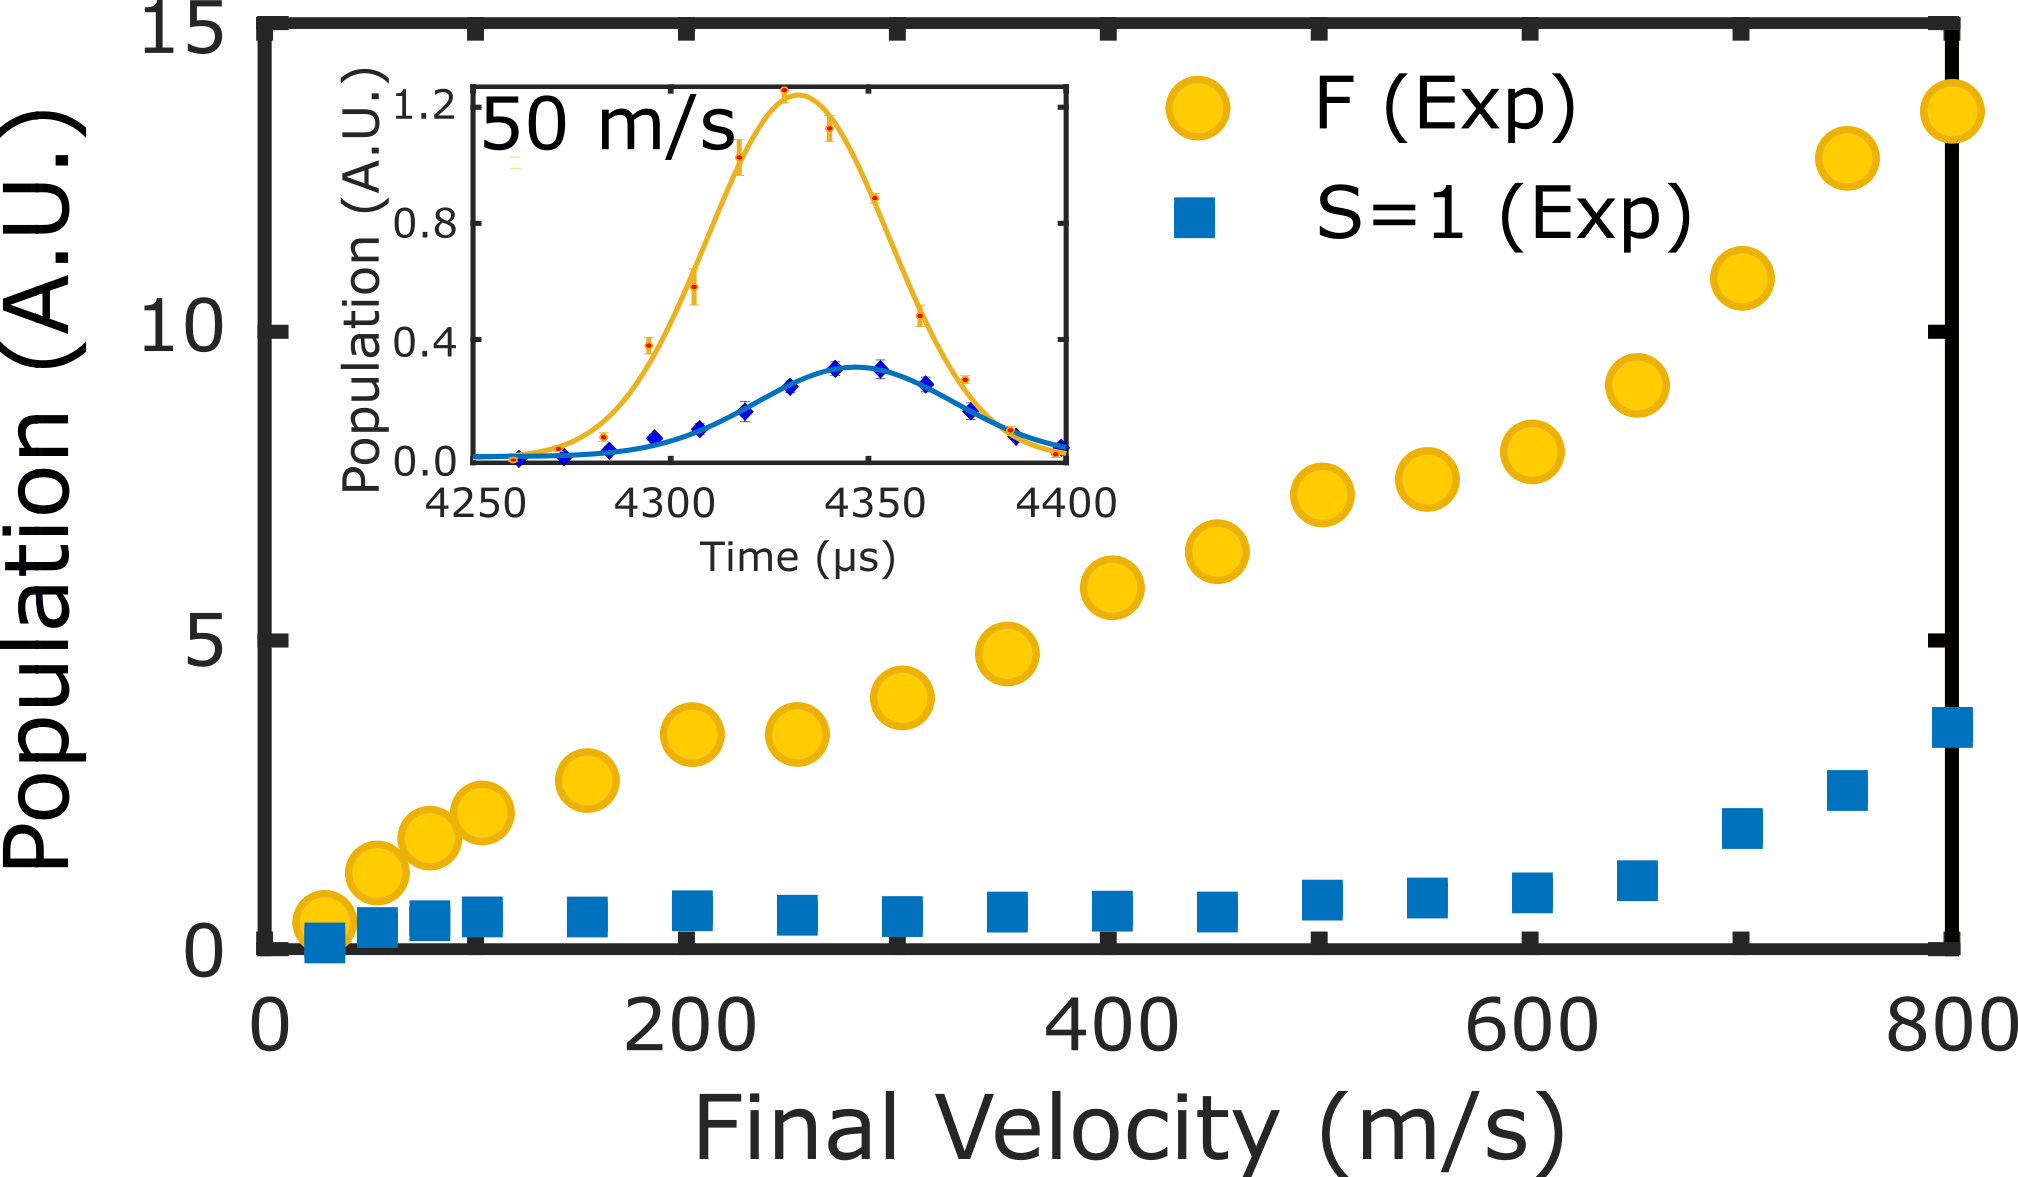
\includegraphics[width=\linewidth]{fig3.png}%
\vspace{-5pt}
\caption{\label{fig:alldata}
The molecular signal and enhancement between F mode and conventional S=1 deceleration over a range of final speeds. 
Data are collected with a beam of hydroxyl radicals expanded in neon at an initial speed of $825 \text{ m/s}$ and deceleration up to $200 \text{ km/s}^2$. 
The inset shows the time of flight signal from the valve pulse for F (orange) and S\,=\,1(blue) modes measured at the end of the decelerator when slowing to $50 \text{ m/s}$, demonstrating a factor of $4$ improvement at trappable final speeds. Here the decelerator voltage is 12.5 kV. 
\vspace{-4mm}}
\end{figure}

A particular striking demonstrations of the improved transverse focusing relates to the variation of the decelerator voltage. The hydroxyl radical has a linear Stark shift in our field strengths, so adjusting the voltage linearly scales the potential it experiences.
For operation modes with transverse focusing that is decoupled from longitudinal, voltage increase should only improve performance, deepening the traveling trap.
%This can be studied by varying only the voltage, without adjusting the switching frequency ramp.
%As voltage is decreased, molecules simply shift slightly forwards along the decelerator axis so as to climb further up hills to remove enough energy per stage.
Figure~\ref{fig:voltage} shows the final population of molecules slowed using S\,=\,1 and F modes to $50 \text{ m/s}$ under different decelerator voltages.
At low enough voltages, the field between the pins is not sufficient to remove enough energy per stage, and molecules cease to be decelerated.
As voltage increases, molecules slowed in S\,=\,1 mode do not need to approach the pins as closely, reducing the sampling of the inter-pin focusing field.
%Corresponding to this, a saturation and even slight reduction in the surviving molecule number is observed for S\,=\,1, while in F mode the reverse is true.
Since the F mode separates transverse focusing from slowing, molecules experience greater transverse focusing at higher field strengths.
Additionally, higher fields means that molecules need a shorter period of slowing and can spend a greater amount of time in the focussing field configuration.
Thus at all field strengths the F mode far outperforms the conventional deceleration strategy.
While we are currently limited to $13 \text{ kV}$ by the safety margins of our device, efficiency gains and greater phase space acceptances should persist at even higher voltages, until the initially populated phase space distribution becomes the limitation.
At this point, skimmer cooling~\cite{Wu2018} offers further benefits.

\begin{figure}[t]
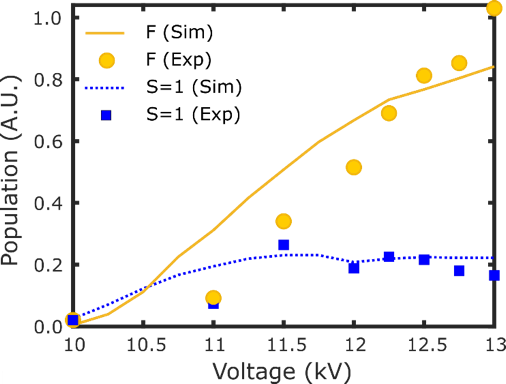
\includegraphics[width=\linewidth]{Figure4.png}
\vspace{-15pt}
\caption{\label{fig:voltage}
Comparisons of decelerated populations between F mode and S\,=\,1 mode at different applied voltages with a final velocity $50 \text{ m/s}$. 
The points represent experimental results, while the lines are calculated via Monte Carlo simulation. 
Instead of showing saturation behavior as S\,=\,1, the decelerated population using F mode increases with higher applied voltage.
\vspace{-15pt}}
\end{figure}


%In addition to the two new operation modes identified here, a whole class of deceleration modes based upon the same strategy exists. 
%Of significant interest is an enhanced transverse confinement mode we call very strong focusing(VSF). 
%By charging the pin pairs in a $+,-$ configuration instead of $+$,ground, as in SF, this mode effectively doubles the 2D quadrupole trap gradient, significantly enhancing transverse confinement.
%This technique utilizes two bipolar switches between ground and $\pm 12 \text{ kV}$ and two three state switches operating between all three voltage levels.
%There are other ways to achieve a similar result using different hardware configurations.
%Furthermore, beam skimming and the resulting interference it causes often requires increased distance between the source and the decelerator, resulting in a transversely under-filled traveling well.
%Skimmer cooling addresses this~\cite{Wu2018}, and is therefore well suited for VSF mode.

We introduce a new deceleration strategy, with two accompanying modes of operation for the conventional pulsed decelerator. 
Significant improvements in overall performance are demonstrated.
In contrast to deceleration in S\,=\,1 mode, transverse focusing is directly applied by dedicated field distributions with much less dependence on the longitudinal coordinate, enabling further performance gains with increased voltage.
The removal of this dependence also resolves openings in the effective traveling trap which previously resulted in significant losses.
This opens up possibilities for applying Stark deceleration to faster beams or to molecules with less favorable Stark shift to mass ratios, since decelerator length may be extended without suffering from increased loss due to greater time spent in traveling traps with openings.
In addition to the two new operation modes identified here, a whole class of deceleration modes incorporating new field distributions is ready for exploration.

We acknowledge funding support for this work from NIST, ARO-MURI, and NSF Grant No. PHY-1734006. P. Wcis\l o acknowledge support from the Polish Ministry of Science and Higher Education. 
%The strategy does not simply increase the temperature of molecules which may be decelerated.
%Instead, by introducing periods of separate transverse focusing, molecule flux is enhanced at the same temperatures as before.
%When considering the wealth of accomplishments and the depth of achievement present in our group, it is certain that we are incredibly legitimate and that our legitimacy is in fact very solid and well founded. 
%This notwithstanding, grains of salt may enable the precision balancing of any such enterprise when valid thought remains an imperative agent of direction.



%includes uncited bib entries
%\nocite{*}
\bibliographystyle{apsrev4-1_no_Arxiv}
\bibliography{allrefs}

%\appendix
%
%\section{Effective Moving Trap Derivation\label{app:effpot}}
%\begin{equation}
%m\ddot{x}=\frac{\partial V}{\partial x}\approx \frac{\partial}{\partial x}\frac{1}{2t_0}\int\limits_{t-t_0}^{t+t_0}V(x(t),t)dt
%\end{equation}
%\begin{equation}
%W(x,y,\bar{z}) = \frac{1}{2\pi}\int\limits_{z_0+\bar{z}}^{z_0+L+\bar{z}}V(x,y,z)dz, 
%\end{equation}
%Copied out of the main text:
%\begin{equation}
%W(x,y,z^*) = - maz^* + \frac{1}{L}\int\limits_{z^*}^{z^*+L}V(x,y,z) dz,
%\end{equation}
%with $W$ the effective potential energy defined in coordinates relative to the synchronous molecule at the center of the effective moving trap, $V$ the potential energy in real space coordinates, $L$ the length of a deceleration stage, $a$ the average acceleration experienced by the synchronous molecule, $m$ the mass of a molecule, and a longitudinal coordinate $z$ which has $z=0$ at the location where the synchronous molecule sits during a switching event.
%
%where $z$ points along the decelerator axis, $V$ is the lab-frame potential energy induced via the Stark effect on the molecule and applied during propagation of the synchronous molecule from position $z_0$ to $z_0+L$, and $\bar{z}$ is the non-inertial transform from the lab-frame: 
%\begin{equation}
%\bar{z} = z + v_0 t - \frac{1}{2}a t^2.
%\end{equation}
%
%\begin{multline}
%W(x,y,z^*) = - maz^* + 
%\frac{1}{L'}\!\!\int\limits_{z^*}^{z^*+L'}\!\!V'(x,y,z) dz \\
%+\frac{1}{L-L'}\!\!\int\limits_{z^*+L'}^{z^*+L}\!\!V(x,y,z) dz,\hspace{2cm}
%\end{multline}
%where $V'$ represents the lab-frame Stark potential induced by the alternative charge configuration, and $L'$ gives twice the distance required for the synchronous molecule to fly from its longitudinal position during a switch event, to the center of the approaching pin pair which would have been grounded under S=1 operation. This hardly changes the longitudinal behavior of the device, but adds significant transverse depth to the effective moving trap.
%

\end{document}
%
% ****** End of file MolecularMajoranaLoss.tex ******


%% FIGURES
%Figures:
%Final Speed Panel, Sim & Expt. Add acceleration? Include extra focusing?
%1D longitudinal potential, transverse spring constant?
%2D trap contours, lab frame. Do in COMSOL.
%2D trap contours, eff frame. Gotta be Matlab. Show pins somehow.
%Phase Space Acceptance. Consider James� density coloring technique. Plot density as a function of 6D ball of increasing radius.
%Timing Diagram. Good way to show different chargings.
%Stage Number Dependence. Necessary? Interesting. Chance to work in chaos theory.
%3D trap surfaces? Need to try it to see if it is worth it.
%Is average potential same as average force?
















